\documentclass[11pt,a4paper,oldfontcommands]{memoir}
\usepackage{ctex}
\usepackage[utf8]{inputenc}
\usepackage[T1]{fontenc}
\usepackage{microtype}
\usepackage[dvips]{graphicx}
\usepackage{xcolor}
\definecolor{linkColor}{RGB}{0, 153, 230}

\usepackage{times}
\usepackage{listings}
\usepackage{courier}
\lstset{
    columns=fixed,       
    numbers=left,                                        % 在左侧显示行号
    frame=none,                                          % 不显示背景边框
    backgroundcolor=\color[RGB]{245,245,244},            % 设定背景颜色
    keywordstyle=\color[RGB]{40,40,255},                 % 设定关键字颜色
    numberstyle=\footnotesize\color{darkgray},           % 设定行号格式
    commentstyle=\color[RGB]{0,96,96},                % 设置代码注释的格式
    stringstyle=\rmfamily\slshape\color[RGB]{128,0,0},   % 设置字符串格式
    showstringspaces=false,                              % 不显示字符串中的空格
    language=c++,                                        % 设置语言
    basicstyle=\small\ttfamily
}

\usepackage[
breaklinks=true,colorlinks=true,
%linkcolor=blue,urlcolor=blue,citecolor=blue,% PDF VIEW
linkcolor=black,urlcolor=black,citecolor=black,% PRINT
bookmarks=true,bookmarksopenlevel=2]{hyperref}

\usepackage{amsmath}
\usepackage{hyperref}

\usepackage{geometry}
% PDF VIEW
% \geometry{total={210mm,297mm},
% left=25mm,right=25mm,%
% bindingoffset=0mm, top=25mm,bottom=25mm}
% PRINT
\geometry{total={210mm,297mm},
left=20mm,right=20mm,
bindingoffset=10mm, top=25mm,bottom=25mm}

\OnehalfSpacing
\chapterstyle{bianchi}
\setsecheadstyle{\Large\bfseries\sffamily\raggedright}
\setsubsecheadstyle{\large\bfseries\sffamily\raggedright}
\setsubsubsecheadstyle{\bfseries\sffamily\raggedright}

\pagestyle{plain}
\makepagestyle{plain}
\makeevenfoot{plain}{\thepage}{}{}
\makeoddfoot{plain}{}{}{\thepage}
\makeevenhead{plain}{}{}{}
\makeoddhead{plain}{}{}{}
\maxsecnumdepth{subsection} % chapters, sections, and subsections are numbered
\maxtocdepth{subsection} % chapters, sections, and subsections are in the Table of Contents

\graphicspath{ {./figure/} }
\begin{document}
\thispagestyle{empty}
{
\sffamily
\centering
{\LARGE
Introduction To 3D Game Programming with DirectX12 笔记
}

\vspace{3.5cm}
(草稿)
\clearpage
\tableofcontents*
\clearpage
\chapter{向量代数(Vector Algebra)}
\chapter{矩阵代数(Matrix Algebra)}
\chapter{矩阵变换(Transformation)}
\chapter{Direct3D 初始化(Direct3D Initialization)}

\chapter{渲染管道(The Rendering Pipeline)}
\section{3D图像(The 3D Illusion)}
\section{模型表达(Model Representation)}
\section{基本计算颜色(Basic Computer Color)}
\begin{flushleft}
计算机显示器在每个像素发射一种混合红、绿、蓝三种颜色的光。当这种混合光到达眼睛并且击中视网膜区域,视锥细胞收到刺激并将产生的神经冲动通过视觉神经传递到大脑。大脑解释这种信号为颜色。随着混合光的变化,使这些视锥细胞收到不同的刺激,从而使大脑中产生不同的颜色。
\end{flushleft}

\subsection{颜色运算(Color Operations)}
\begin{itemize}
    \item 加法:$(0.0, 0.5, 0) + (0, 0.0, 0.25) = (0.0, 0.5, 0.25)$
    \item 减法:$(1, 1, 1) - (1, 1, 0) = (0, 0, 1)$
    \item 标量乘法:$0.5(1, 1, 1) = (0.5, 0.5, 0.5)$
    \item 显然,点乘和叉乘对于颜色向量来说没有意义。然而,颜色向量有一特殊的运算称为调制或分量乘法:$(c_{r},c_{g},c_{b}) \otimes (k_{r},k_{g},k_{b}) = (c_{r}k_{r},c_{g}k_{g},c_{b}k_{b})$。该运算主要用来作为照明方程。举个例子,假设我们有一束入射光线(r,g,b),它会照射一个反射50%红光,75%绿光和25%蓝光的表面,并吸收剩余的光线。 然后反射光线的颜色由下式给出:$(r,g,b) \otimes (0.5,0.75,0.25) = (0.5r,0.75g,0.25b)$
\end{itemize}

\subsection{128位颜色(128-Bit Color)}
\begin{flushleft}
通常我们会合并另外的颜色分量,称作 alpha 分量。alpha 分量常用来表示颜色的透明度(透明度在混合中很有用,因为我们还没有使用混合,目前只需将 alpha 分量设为 1 即可)。包含 alpha 分量意味着我们用 4D 颜色向量$(r, g, b, a), 0 \leq r,g,b,a \leq 1$ 为了用 128-bits 表示一种颜色,每个分量使用浮点型值。因为数学上,一种颜色就是一个 4D 向量,我们能在代码中使用 XMVECTOR 类型来表示一种颜色,并且每当调用 DirectX Math 中的向量函数时都会受益于 SIMD (如,颜色加减和标量乘法)。为了方便分量乘法,DirectX Math 库提供了下面方法:
\begin{lstlisting}
// Return c1 \otimes c2
XMVECTOR XM_CALLCONV XMColorModulate(FXMVECTOR C1, FXMVECTOR C2);
\end{lstlisting}
\end{flushleft}

\subsection{32位颜色(32-Bit Color)}
\begin{flushleft}
要以32位大小来表示一个颜色,可以给每个分量分配一个字节(8-bit)大小。这样一来,每个分量最多能表现256种色调——0代表无强度,255代表满强度,中间值代表中间强度。看似每个分量一个字节很小,但是组合在一起$(256 \times 256 \times 256)$就表示百万种不同的颜色。DirectX Math 库(\#include <DirectXPackedVector.h>) DirectX::PackedVector 命名空间(namespace)下提供了以下数据结构来存储32位颜色:
\begin{lstlisting}
namespace DirectX
{
namespace PackedVector
{
    // ARGB Color; 8-8-8-8 bit unsigned normalized integer components packed
    // into a 32 bit integer. The normalized color is packed into 32 bits
    // using 8 bit unsigned, normalized integers for the alpha, red, green,
    // and blue components.
    // The alpha component is stored in the most significant bits and the
    // blue component in the least significant bits (A8R8G8B8):
    // [32] aaaaaaaa rrrrrrrr gggggggg bbbbbbbb [0]
    struct XMCOLOR
    {
        union
        {
            struct
            {
                uint8_t b; // Blue: 0/255 to 255/255
                uint8_t g; // Green: 0/255 to 255/255
                uint8_t r; // Red: 0/255 to 255/255
                uint8_t a; // Alpha: 0/255 to 255/255
            };
            uint32_t c;
        };
        XMCOLOR() {}
        XMCOLOR(uint32_t Color) : c(Color) {}
        XMCOLOR(float _r, float _g, float _b, float _a);
        explicit XMCOLOR(_In_reads_(4) const float *pArray);
        operator uint32_t () const { return c; }
        XMCOLOR& operator= (const XMCOLOR& Color) 
        { c = Color.c; return *this; }
        XMCOLOR& operator= (const uint32_t Color) 
        { c = Color; return *this; }
    };
} // end PackedVector namespace
} // end DirectX namespace
\end{lstlisting}
一个32位颜色数据能被转换为128位颜色数据: 将整数区间$[0, 255]$ 映射到实数区间$[0, 1]$。每个数除以255即可,也就是说 设$0 \leq n \leq 255$,且 n 是整数,则 $0 \leq \frac{n}{255} \leq 1$ 就是需要的范围 0 到 1 的颜色强度。例:(80,140,200,255)转换如下:
$$ (80,140,200,255)\rightarrow (\frac{80}{255},\frac{140}{255},\frac{200}{255},\frac{255}{255}) \approx (0.31,0.55,0.78,1.0)$$
另一方面,128位颜色能转换为32位颜色:将每个分量乘以255并且四舍五入取整。例:
$$(0.3,0.6,0.9,1.0)\rightarrow (0.3\cdot 255,0.6\cdot 255,0.9\cdot 255,1.0\cdot 255)=(77,153,230,255)$$

在将32位颜色转换为128位颜色时通常必须执行额外的位操作,反之,因为8位颜色组件通常打包为32位整数值(如 unsigned int),XMCOLOR 就是如此。DirectXMath 库定义了一个方法以 XMCOLOR 作为参数,返回XMVECTOR:
\begin{lstlisting}
XMVECTOR XM_CALLCONV PackedVector::XMLoadColor(const XMCOLOR* pSource);
\end{lstlisting}
\end{flushleft}

\subsection{渲染管道概览(Overview of the rendering pipeline)}
\subsection{输入汇编程序阶段(The Input Assembler Stage)}
\subsubsection{顶点(Vertices)}
\subsubsection{原始拓扑(Primitive Topology)}
\subsubsection{指数(Indices)}
\subsection{顶点着色器阶段(The Vertex Shader Stage)}
\subsubsection{局部空间和世界空间(Local Space and World Space)}
TODO
\subsubsection{视图空间(View Space)}
\begin{flushleft}
为了形成场景的二维图像,我们必须在场景中放置一个虚拟相机。 相机指定了观众可以看到的世界的多大的体积,以及我们需要生成多大的世界体积来生成二维图像。让我们将一个局部坐标系统(称为视图空间,眼图空间或相机空间)附加到相机,如图\ref{fig:5-19}所示; 也就是说,摄像机坐落在正视z轴的原点处,x轴指向摄像机的右侧,y轴指向摄像机的上方。 而不是描述相对于世界空间的场景顶点,基于相机坐标系,渲染管线的后面阶段很方便地描述它们。从世界空间到视图空间的坐标变换称为视图变换,相应的矩阵称为视图矩阵。\\
\begin{figure}[t]
    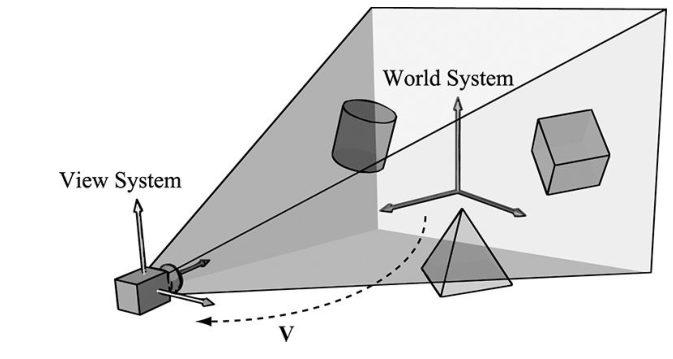
\includegraphics[width=\textwidth]{5-19}
    \centering
    \caption{转换顶点相对于世界空间的坐标,使它们相对于相机空间。}
    \label{fig:5-19}
\end{figure}
如果$Q_{w}=(Q_{x},Q_{y},Q_{z},1)$,$u_{w}=(u_{x},u_{y},u_{z},0)$,$v_{w}=(v_{x},v_{y},v_{z},0)$,$w_{w}=(w_{x},w_{y},w_{z},0)$分别用相对于世界空间的齐次坐标来描述视图空间的原点,x轴,y轴和z轴,然后我们从3.4.3一节知道坐标矩阵从视图空间的变化到世界空间是:
$$W=
\begin{bmatrix}
u_{x} & u_{y} & u_{z} & 0\\
v_{x} & v_{y} & v_{z} & 0\\
w_{x} & w_{y} & w_{z} & 0\\
Q_{x} & Q_{y} & Q_{z} & 1
\end{bmatrix}$$\\
然而,这不是我们想要的转换。我们想要的是倒置转换,即从世界空间转换成视图空间。回忆3.4.3节,倒置转换就是求矩阵的逆。因此$W^{-1}$就是从世界空间到视图空间的转换。\\
世界坐标系统和视图坐标系统仅在位置和方向有区别,所以直观地得到 $W=RT$(也就是说世界矩阵能被分解为一个旋转跟一个平移(translation))\footnote{$R$是\href{https://en.wikipedia.org/wiki/Orthogonal_matrix}{\textcolor{linkColor}{正交矩阵}},所以有 $R^{-1}=R^{T}$}。这让求逆变得简单:
\begin{align*}
V&=W^{-1}=(RT)^{-1}=T^{-1}R^{-1}=T^{-1}R^{T} \\
&=\begin{bmatrix}
1 & 0 & 0 & 0\\
0 & 1 & 0 & 0\\
0 & 0 & 1 & 0\\
-Q_{x} & -Q_{y} & -Q_{z} & 1
\end{bmatrix}
\begin{bmatrix}
u_{x} & v_{x} & w_{x} & 0\\
u_{y} & v_{y} & w_{y} & 0\\
u_{z} & v_{z} & w_{z} & 0\\
0 & 0 & 0 & 0
\end{bmatrix} \\
&=\begin{bmatrix}
u_{x} & v_{x} & w_{x} & 0\\
u_{y} & v_{y} & w_{y} & 0\\
u_{z} & v_{z} & w_{z} & 0\\
\mathbf{-Q\cdot u} & \mathbf{-Q\cdot v} & \mathbf{-Q\cdot w} & 1
\end{bmatrix}
\end{align*}

所以,视图矩阵就是:
\begin{align*}
V=\begin{bmatrix}
u_{x} & v_{x} & w_{x} & 0\\
u_{y} & v_{y} & w_{y} & 0\\
u_{z} & v_{z} & w_{z} & 0\\
\mathbf{-Q\cdot u} & \mathbf{-Q\cdot v} & \mathbf{-Q\cdot w} & 1
\end{bmatrix}
\end{align*}
现在我们用一种直观的方式来构造向量,这些向量用来建立视图矩阵。令\textbf{Q}为摄像机的位置,\textbf{T}为摄像机对准的目标点。然后,令\textbf{j}为世界空间向上方向的单位向量。(本书中,世界坐标系的 xz 构成的平面作为世界地平面,世界 y 轴描述了向上的方向;所以,$j=(0,1,0)$ 就是和世界 y 轴平行的单位向量。然而这只是约定,一些应用可能会选择 xy构成的平面作为地平面,z轴作为向上方向。)参考图片\ref{fig:5-20},摄像机的朝向如下:
$$w=\frac{T-Q}{||T-Q||}$$
该向量描述的是摄像机的z轴,对准\textbf{w}右侧的单位向量:\\
$$u=\frac{j\times w}{||j \times w||}$$
该向量描述的是摄像机的 x 轴。最后,摄像机的y轴单位向量为:\\
$$v=w \times u$$
因为\textbf{w}和\textbf{u}是互相正交的单位向量,$w\times u$也必定是单位向量,没必要正规化。\\
综上所述,给定摄像机的位置,目标点,和世界向上方向,我们就能求得摄像机的本地坐标系统,作为视图矩阵。
\begin{figure}[t]
    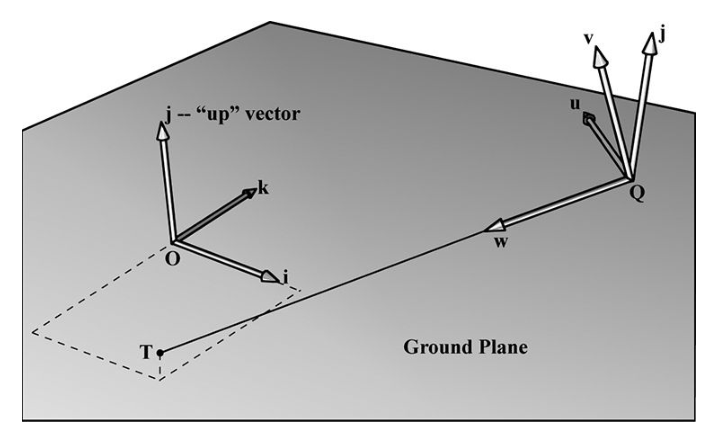
\includegraphics[width=\textwidth]{5-20}
    \centering
    \caption{根据相机位置,目标点和世界“向上”矢量构造相机坐标系。}
    \label{fig:5-20}
\end{figure}

DirectXMath 库提供了计算视图矩阵的方法:
\begin{lstlisting}
// Outputs view matrix V
XMVECTOR XM_CALLCONV XMMatrixLookAtLH(
    FXMVECTOR EyePosition,    // Input camera position Q
    FXMVECTOR FocusPosition,  // Input target point T
    FXMVECTOR UpDirection);   // Input world up direction j
\end{lstlisting}
通常世界y轴就是向上的方向,所以$j=(0,1,0)$ 就是向上的向量。例:假设我们将摄像机放在相对于世界坐标的$(5,3,-10)$处,并且对准世界原点坐标$(0,0,0)$。可以通过下面方式获得视图矩阵:\\
\begin{lstlisting}
XMVECTOR pos    = XMVectorSet(5, 3, -10, 1.0f);
XMVECTOR target = XMVectorZero();
XMVECTOR up     = XMVectorSet(0.0f, 1.0f, 0.0f, 0.0f);
XMMATRIX V      = XMMatrixLookAtLH(pos, target, up);
\end{lstlisting}
\end{flushleft}
\subsubsection{投影和齐次裁剪空间(Projection and Homogeneous Clip Space)}
\begin{flushleft}
到目前为止我们描述了在世界空间中摄像机的位置和方向,但摄像机还有一个部分需要解决,即摄像机看到的空间体积。体积由视锥来描述(见图\ref{fig:5-21})。
\end{flushleft}
\begin{figure}[t]
    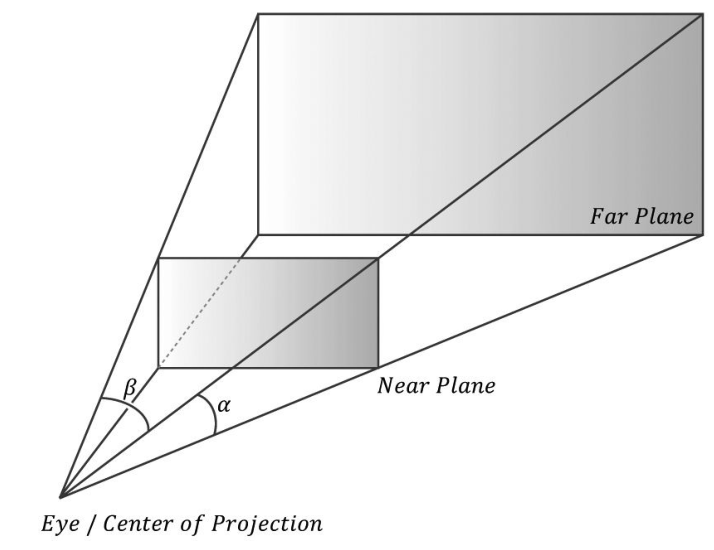
\includegraphics[width=\textwidth]{5-21}
    \centering
    \caption{视锥定义了摄像机“看到”的空间体积}
    \label{fig:5-21}
\end{figure}
\begin{flushleft}
我们接下来的任务是将一个 3D 几何体在视锥中投影到 2D 投影窗口中。投影必须以平行线汇聚到消失点的方式完成,当一个物体的3D深度增加(距离拉远),投影的大小就减小。这就是\href{https://en.wikipedia.org/wiki/Perspective_(graphical)}{\textcolor{linkColor}{透视投影}}(如图\ref{fig:5-22})。我们将一个顶点到视点(眼睛所在的位置,姑且叫视点吧)的连线称为顶点的投影线。然后我们定义透视投影变换就是3D顶点\textbf{v}变换成它的投影线和2D投影面板交叉点\textbf{v'}的过程;我们认为\textbf{v'}就是\textbf{v}的投影。一个3D物体的投影就是组成这个物体的所有顶点的投影。
\end{flushleft}
\begin{figure}[t]
    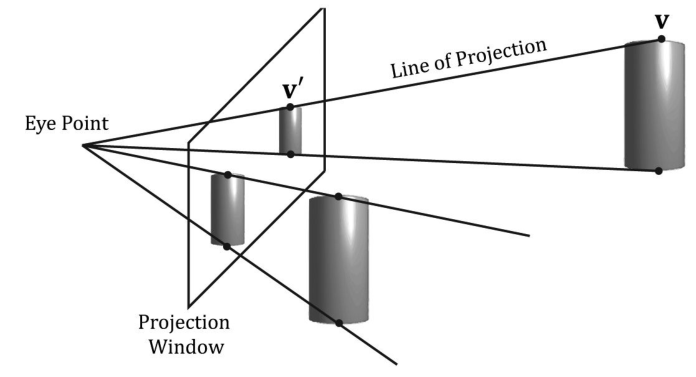
\includegraphics[width=\textwidth]{5-22}
    \centering
    \caption{两个圆柱体大小相同,但深度不同。距离眼睛近的圆柱体比距离远的圆柱体投影大。视锥中的几何体被投影到投影窗口;视锥外的集合体,投影到投影面板上,但在投影窗口外面(投影面板和投影窗口共面)}
    \label{fig:5-22}
\end{figure}

\paragraph{定义一个视锥(Defining a Frustum)}
\begin{flushleft}
我们可以在视图空间中定义一个视锥,其投影中心位于原点处,并沿着正z轴向下看,通过以下四个量:近平面$n$,远平面$f$,垂直视场角$\alpha$ 和纵横比 $r$。请注意,在视图空间中,近平面和远平面平行于$xy$平面; 因此我们只需指定它们沿着z轴的原点距离。 纵横比由 $r=w/h$ 定义,其中$w$是投影窗口的宽度,$h$是投影窗口的高度(视图空间中的单位)。 投影窗口本质上是视图空间中场景的二维图像。 这里的图像最终将映射到后台缓冲区(back buffer); 因此,我们喜欢投影窗口尺寸的比率与后台缓冲区尺寸的比率相同。所以后缓冲区维度的比率通常被指定为长宽比(这是一个比例,所以它没有单位)。例,如果后台缓冲区尺寸是 $800 \times 600$,则 $r=\frac{800}{600} \approx 1.333$。如果投影窗口与后台缓冲区的纵横比不相同,则需要非均匀缩放来将投影窗口映射到后台缓冲区,这将导致失真(例如,投影窗口上的圆圈可能当映射到后台缓冲区时被拉伸成一个椭圆)。\\
我们将水平视角标记为$\beta$,垂直视角标记为$\alpha$,纵横比为$r$。要看看$r$如何帮助我们找到$\beta$,请考虑图\ref{fig:5-23}。 请注意,投影窗口的实际尺寸并不重要,只需要保持纵横比。 因此,我们会选择2的方便高度,因此宽度必须为:\\
$$r=\frac{w}{h}=\frac{w}{2}\Rightarrow w=2r$$
\end{flushleft}
\begin{figure}[t]
    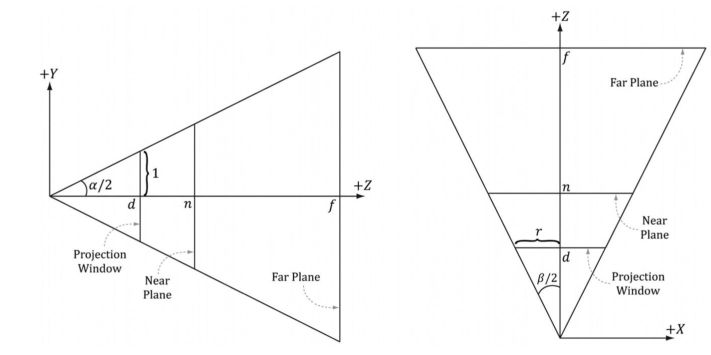
\includegraphics[width=\textwidth]{5-23}
    \centering
    \caption{给定垂直视角$\alpha$和纵横比$r$,得出水平视角$\beta$}
    \label{fig:5-23}
\end{figure}
\begin{flushleft}
为了具有指定的垂直视场$\alpha$,投影窗口必须放置在距离原点的距离$d$处:
$$\tan(\frac{\alpha}{2})=\frac{1}{d}\Rightarrow d=\cot(\frac{\alpha}{2})$$
现在我们已经将投影窗沿$z$轴的距离d固定为当投影窗的高度为2时垂直视场$\alpha$。现在我们可以求解$\beta$。 看一下图\ref{fig:5-23}中的$xz$平面,我们现在看到:
$$\tan(\frac{\beta}{2})=\frac{r}{d}=\frac{r}{\cot(\frac{\alpha}{2})}=r\cdot \tan(\frac{\alpha}{2})$$
因此,考虑到垂直视角α和纵横比r,我们总能得到水平视角β:
$$\beta=2\tan^{-1}(r\cdot\tan(\frac{\alpha}{2}))$$
\end{flushleft}

\paragraph{投影顶点(Projecting Vertices)}
\begin{figure}[t]
    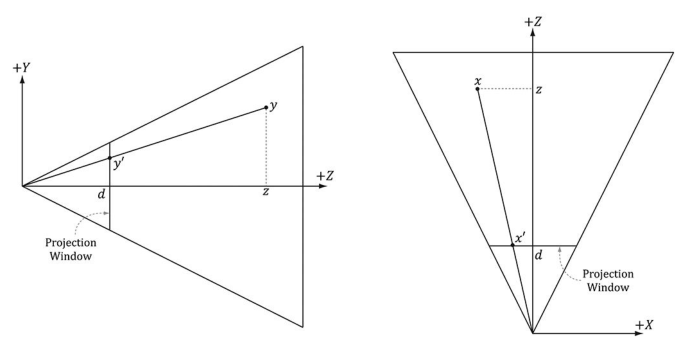
\includegraphics[width=\textwidth]{5-24}
    \centering
    \caption{相似三角}
    \label{fig:5-24}
\end{figure}
\begin{flushleft}
参考图\ref{fig:5-24}。 给定一个点$(x,y,z)$,我们希望在投影平面$z = d$上找到它的投影$(x',y',d)$。 通过分别考虑$x$和$y$坐标并使用相似的三角形,我们发现:
\begin{align*}
\frac{x'}{d}=\frac{x}{z}\Rightarrow x'=\frac{xd}{z}=\frac{x\cot(\alpha/2)}{z}=\frac{x}{z\tan(\alpha/2)}\\
\frac{y'}{d}=\frac{y}{z}\Rightarrow y'=\frac{yd}{z}=\frac{y\cot(\alpha/2)}{z}=\frac{y}{z\tan(\alpha/2)}\\
\end{align*}
显然对于点$(x,y,z)$, $-r\leq x'\leq r,-1\leq y'\leq 1,n\leq z\leq f$
\end{flushleft}

\paragraph{标准化的设备坐标(Normalized Device Coordinate-NDC)}
\begin{flushleft}
上一节中投影点的坐标是在视图空间中计算的。 在视图空间中,投影窗口的高度为2,宽度为$2r$,其中$r$是纵横比。 问题在于,尺寸取决于宽高比。 这意味着我们需要告诉硬件高宽比,因为硬件稍后需要做一些涉及投影窗口尺寸的操作(比如将其映射到后台缓冲区)。 如果我们能够消除这种对长宽比的依赖性会更方便。 解决的办法是将投影的$x$坐标从区间$[-r,r]$缩放到$[-1,1]$像这样:
\begin{align*}
-r\leq x' \leq r \\
-1\leq x'/r \leq 1
\end{align*}

在映射之后,$x$坐标和$y$坐标被称为标准化的设备坐标(NDC)(z坐标还没有被标准化),并且点$(x,y,z)$在视锥内当且仅当:
\begin{align*}
-1\leq x'/r \leq 1 \\
-1\leq y' \leq 1 \\
n \leq z \leq f
\end{align*}

从视图空间到NDC空间的转换可视为单位转换。 我们有一个关系,即一个NDC单位在$x$轴上等于视图空间中的$r$个单位(即 1ndc = \textbf{r} vs)。 所以给定$x$个视图空间单位,我们可以使用这个关系来转换单位:
$$x\mathit{vs}\cdot \frac{1\mathit{ndc}}{r\mathit{vs}}=\frac{x}{r}\mathit{ndc}$$
我们可以修改我们的投影公式,直接在NDC坐标中为我们提供投影的$x$坐标和$y$坐标:
\begin{align*}\tag{eq.5.1}\label{eq.5.1}
x'&=\frac{x}{rz\tan(\alpha/2)}\\
y'&=\frac{y}{z\tan(\alpha/2)}
\end{align*}
请注意,在NDC坐标中,投影窗口的高度为2,宽度为2.因此,现在尺寸是固定的,硬件无需知道纵横比,但我们有责任始终在NDC中提供投影坐标空间(图形硬件假设我们会)。
\end{flushleft}

\paragraph{用矩阵来描述投影公式(Writing the Projection Equations with a Matrix)}
\begin{flushleft}
为了保持一致,我们将用一个矩阵来描述投影变换。不过,公式\ref{eq.5.1}是非线性的,无法用矩阵描述。所以我们要使用一种“技巧”将它分为两部分来实现:一个线性部分和一个非线性部分。非线性部分要除以$z$。我们会在下一节讨论“如何规范化$z$坐标”时讲解这一问题;现在读者只需要知道,我们会因为个除法操作而失去原始的z坐标。所以,我们必须在变换之前保存输入的z坐标;我们可以利用齐次坐标来解决一问题,将输入的$z$坐标复制给输出的$w$坐标。在矩阵乘法中,我们要将元素[2][3]设为1、元素[3][3]设为0(从0开始的索引)。我们的投影矩阵大致如下:
\begin{align*}
P=\begin{bmatrix}
\frac{1}{r\tan(\alpha/2)} & 0 & 0 & 0\\
0 & \frac{1}{\tan(\alpha/2)} & 0 & 0\\
0 & 0 & A & 1\\
0 & 0 & B & 0
\end{bmatrix}
\end{align*}
注意矩阵中的常量$A$和$B$(它们将在下一节讨论);这些常量用于把输入的$z$坐标变换到规范化区间。将一个任意点$(x,y,z,1)$与该矩阵相乘,可以得到:
\begin{align*}\tag{eq.5.2}\label{eq.5.2}
[x,y,z,1]\begin{bmatrix}
\frac{1}{r\tan(\alpha/2)} & 0 & 0 & 0\\
0 & \frac{1}{\tan(\alpha/2)} & 0 & 0\\
0 & 0 & A & 1\\
0 & 0 & B & 0
\end{bmatrix}=\left[ \frac{x}{r\tan(\alpha/2)},\frac{y}{\tan(\alpha/2)},Az+B,z\right]
\end{align*}
在与投影矩阵(线性部分)相乘之后,我们要将每个坐标除以$w = z$(非线性部分),得到最终的变换结果:
\begin{align*}\tag{eq.5.3}\label{eq.5.3}
\left[ \frac{x}{r\tan(\alpha/2)},\frac{y}{\tan(\alpha/2)},Az+B,z\right]
\xrightarrow[]{\text{除以$w$}}
\left[ \frac{x}{rz\tan(\alpha/2)},\frac{y}{z\tan(\alpha/2)},A+\frac{B}{z},1\right]
\end{align*}
顺便提一句,你可能会问:“如何处理除数为0的情况”;对于一问题我们不必担心,因为近平面总是大于0的,其他的点都会被裁剪掉(参见5.9节)。有时,与$w$相除的过程也称为透视除法(perspective divide)或齐次除法(homogeneous divide)。我们可以看到$x$、$y$的投影坐标与公式\ref{eq.5.1}相同。
\end{flushleft}
\end{document}
